\subheading{Wherein the Cart System\\ is Identified}
\section*{Section Four (a)}

Now that the function to identify the system had been developed, tested and
found to be accurate the actual characterisation of the cart could begin.  The
characterisation simply involved taking in the provided datasets and running them
through the identification function.  This resulted in a $C$ and $b$ value for
each frequency at which the system was tested.  As instructed the values derived
from the seventh data set with a frequency of 1.8 Hz was used as the general
model.  The results of this identification were a $C$ value of $5.83523$ and a
$\beta$ vale of $1.93596$.

\subheading{Wherein the Identification\\ is Ridiculed}
\section*{Section Four (b)}

To check the results of the identification the model was used to generate data
at all 12 frequencies tested and this generated data was compared to the
measurements.  The comparison was performed by finding the absolute difference
between the generated data and the measured data for each frequency, scaling
this difference by the mean of the absolute measured data for that frequency and
finally finding the median and 90\% confidence interval of the relative error.

Figure and Table \ref{4b} shows these medians and the 90\% confidence interval
found.  Obviously the model is most accurate at the frequency it was derived
from, the relative error is down to 0--6\% showing the very good accuracy.  The
worst case is at $f = 2.6$, $\omega = 16.3$ with a 90\% CI of the error in the
range 0--63\%, this is obviously an unacceptable level of error so the model is
really only valid for the one frequency it was derived for, and maybe the ones
either side depending on the use case.

The relative errors from each frequency were then concatenated and the median
and 90\% CI of the overall error was calculated.  This came out to a median
error of 0.21840 and a 90\% CI of 0--49\%.  Again a most likely case of 22\%
error and a worst case of around 49\% error is likely unacceptable for the
majority of use cases of this model.


Figure \ref{4b-2-fig} shows a histogram of the error values.  Looking at this
the bell shape of a Gaussian distribution can be easily seen.

\begin{figure}
  \centering
  \begin{minipage}{0.4\textwidth}
    \centering\scriptsize
    \begin{tabular}{c|c|c}
        Frequency & Relative Median error & 90\% CI \\
        \hline
        0.6 & 0.26936 & 0.26175 \\
        0.8 & 0.30116 & 0.25065 \\
        1.0 & 0.32473 & 0.24677 \\
        1.2 & 0.31176 & 0.23621 \\
        1.4 & 0.24266 & 0.20618 \\
        1.6 & 0.11872 & 0.12534 \\
        1.8 & 0.02376 & 0.03305 \\
        2.0 & 0.11852 & 0.13654 \\
        2.2 & 0.18552 & 0.21159 \\
        2.4 & 0.22813 & 0.21008 \\
        2.6 & 0.28859 & 0.32453 \\
        2.8 & 0.28994 & 0.28366 
    \end{tabular}
  \end{minipage}
  \hspace{0.1\textwidth}
  \begin{minipage}{0.4\textwidth}
    \centering
    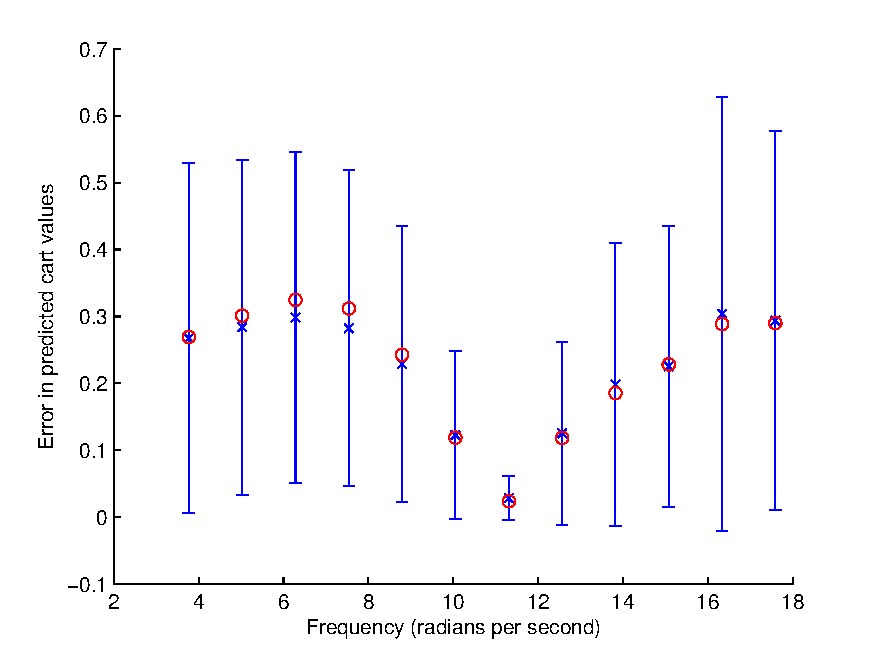
\includegraphics[width=\textwidth]{images/section-4b}
  \end{minipage}
  \caption{Error in the derived model\label{4b}}
\end{figure}

\includefigure{width=0.6\textwidth}
              {images/section-4b-2}
              {Histogram of the error values\label{4b-2-fig}}
